\documentclass{article}
\usepackage[a4paper, left=1.5cm, right=1.5cm, top=1cm, bottom=2cm]{geometry}
\usepackage{tikz,tcolorbox}
\usepackage{amsmath}
\usepackage[table,xcdraw]{xcolor}
\usepackage{listings}
\usepackage{array,multirow} % For customizing tables
\usepackage{booktabs} % For better horizontal lines
\usepackage{makecell}
\usepackage[colorlinks=true, linkcolor=blue, urlcolor=blue]{hyperref}
\setlength{\parindent}{0pt}

\usepackage{amssymb}
\tcbuselibrary{skins, breakable, theorems}

\definecolor{myblue}{HTML}{10C2C4}

\newtcolorbox{prettyBox}[2]{
  enhanced,
  colback=white!90!#2,   % Background color based on the second parameter (color)
  colframe=#2!60!black,  % Frame color based on the second parameter (color)
  coltitle=white,        % Title color (white)
  fonttitle=\bfseries\Large,
  title=#1,              % Title from the first parameter
  boxrule=1mm,
  arc=0.5mm,
  drop shadow=#2!35!gray, % Drop shadow color based on the second parameter (color)
}

\usepackage{listings}
% Define the style for C code
\lstdefinestyle{cstyle}{
    language=C,
    basicstyle=\ttfamily\small,
    keywordstyle=\color{blue}\bfseries,
    stringstyle=\color{red},
    commentstyle=\color{green!50!black}\itshape,
    numbers=left,
    numberstyle=\tiny\color{gray},
    stepnumber=1,
    breaklines=true,
    frame=tb,
    tabsize=4,
    showstringspaces=false,
    captionpos=b
}

\lstdefinestyle{cmd}{
 basicstyle=\ttfamily,
 backgroundcolor=\color{lightgray!20},
 frame=single
}

\lstdefinestyle{javaStyle}{
    language=Java,
    basicstyle=\ttfamily\footnotesize,   % Font style and size
    numbers=left,                       % Line numbers on the left
    numberstyle=\tiny\color{gray},       % Style for line numbers
    stepnumber=1,                        % Line number step
    numbersep=5pt,                       % Distance of numbers from the code
    backgroundcolor=\color{white},       % Background color of the listing
    showspaces=false,                    % Don't show spaces
    showstringspaces=false,              % Don't show spaces in strings
    showtabs=false,                      % Don't show tab characters
    frame=single,                        % Add a frame around the code
    rulecolor=\color{black},             % Color of the frame
    tabsize=2,                           % Tab size
    captionpos=b,                        % Position of the caption (bottom)
    breaklines=true,                     % Automatically break long lines
    breakatwhitespace=true,              % Break at white space
    escapeinside={\%*}{*)},              % Allows comments in LaTeX inside the listing
    keywordstyle=\color{blue},           % Keyword color
    commentstyle=\color{green},          % Comment color
    stringstyle=\color{red},             % String color
}



\lstdefinestyle{pythonstyle2}{
    language=python,                    % Language set to Python
    basicstyle=\ttfamily\footnotesize,   % Change basic font size
    keywordstyle=\color{blue}\bfseries, % Different keyword style
    stringstyle=\color{red},         % Different string color
    commentstyle=\color{green!60!black}\itshape, % Adjust comment color
    numbers=left,                       % Line numbers on the left
    numberstyle=\tiny\color{gray},      % Smaller number font and color
    stepnumber=1,                       % Number each line
    frame=single,                       % Single frame around code
    tabsize=4,                          % Adjust tab size
    showstringspaces=false,             % Do not show spaces in strings
    captionpos=b,% Position of caption
    breaklines=true,
    inputencoding=utf8
}

\newcommand{\tit}[1]{
\begin{center}
    \Large{\textbf{{#1}}}
\end{center}
}




\begin{document}

\tit{TP N\(^{\boldsymbol{\circ}}\)\hspace{0.1cm}1}


\vspace{0.75cm}

The includes needed
\begin{itemize}
    \item stdio.h : to printf and get user input
    \item stdlib.h : to use exit to terminate whole 
programe and to terminate child process
    \item unistd.h :to use fork and pipe primitive
    \item ctype.h : to use toupper function
    \item sys/wait.h : to use wait primitive (parent wait for child to terminate)
\end{itemize}
\newpage
\lstinputlisting[style=cstyle,basicstyle=\footnotesize\ttfamily]{Questions/EX1/ex1Overview.c}

child\_1 void function :
\lstinputlisting[style=cstyle,firstline=10,lastline=33,basicstyle=\footnotesize\ttfamily]{Questions/EX1/ex1.c}

\vspace{0.5cm}

child\_2 void function :
\lstinputlisting[style=cstyle,firstline=36,lastline=50,basicstyle=\footnotesize\ttfamily]{Questions/EX1/ex1.c}



\begin{center}
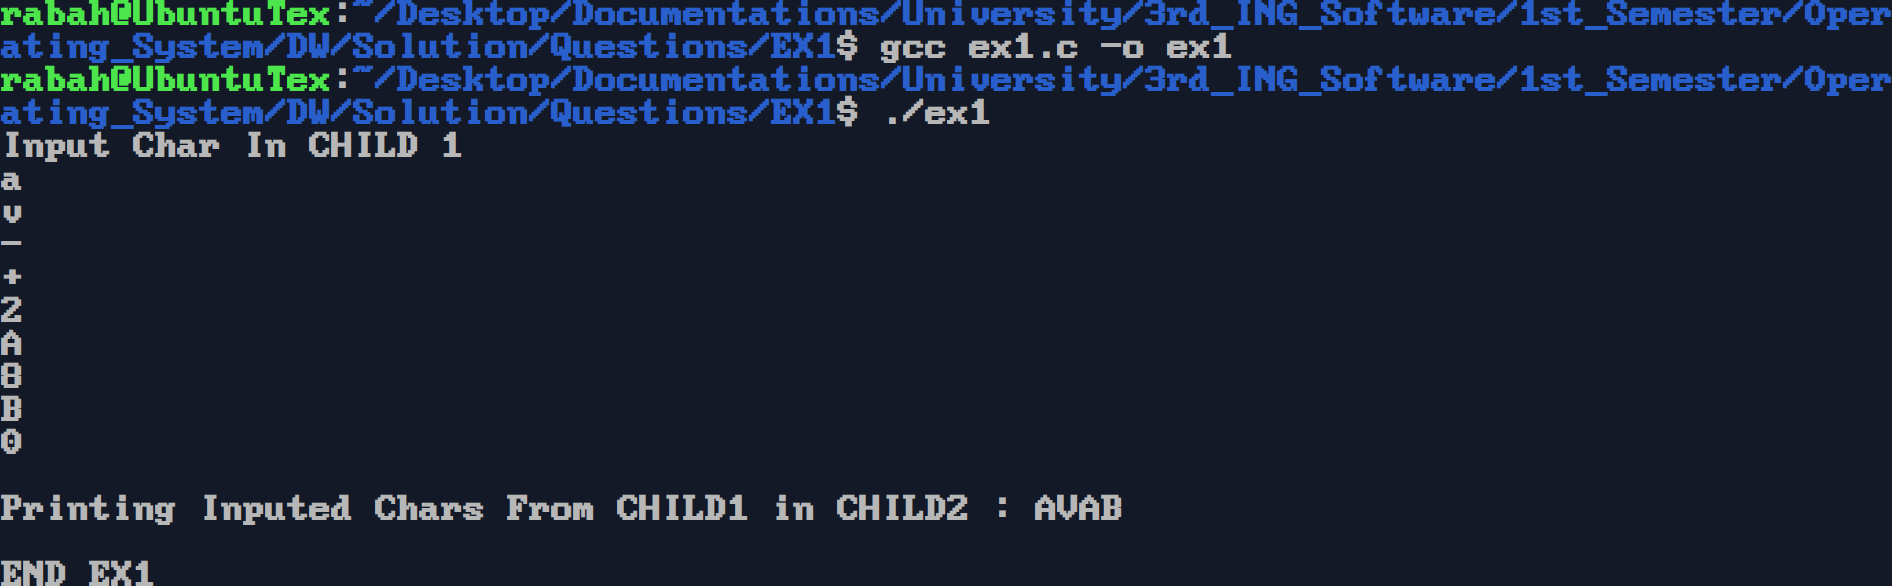
\includegraphics[width=\textwidth]{Questions/EX1/output.png}
\end{center}


\subsubsection*{\underline{Experimental}}
\begin{tabular}{|c|c|c|c|c|c|c|c|c|c|c|c|c|c|c|}
    \hline
    N & \(10^3\) & \(2.10^3\) & \(10^4\) & \(2.10^4\) & \(10^5\) & \(2.10^5\) & \(10^6\) & \(2.10^6\) & \(10^7\) & \(2.10^7\) & \(10^8\) & \(2.10^8\) & \(10^9\) & \(2.10^9\) \\
    \hline
    \makecell{Time\\\((10^{-5})\)} & 8 & 9.8 & 10.8 & 19.4 & 33.6 & 59.3 & 261.1 & 505.7 & 2458.4 & 5071.6 & 24458.7 & 48759.0 & 243312.2 & 487828.6 \\
    \hline
\end{tabular}



\vspace{1cm}

\newpage

\subsubsection*{\underline{Theoritical}}
We first need to find  \(\Delta t\) , for that we will take one runtime value from the experimental study and solve a simple equation 

\vspace{0.15cm}

for n = \(10^4\) and execution time T(n) = \(10.8\times10^{-5}\) :

\vspace{0.75cm}
\begin{align*}
&f(n)\times\Delta t = T(n)\\[0.15cm]
&\Delta t = \frac{T(n)}{f(n)} \\[0.15cm]
&\Delta t = \frac{T(n)}{5n + 6}\\[0.15cm]
&\Delta t = \frac{10.8\times10^{-5}}{5\times 10^4 + 6} \\[0.15cm]
&\Delta t = 2.1597408311\times10^{-9} \\[0.25cm]
&\boxed{\Delta t \approx 2.16\times10^{-9}}
\end{align*}





\vspace{2cm}
\begin{tabular}{|c|c|c|c|c|c|c|c|c|c|c|c|c|c|c|c|c|}
    \hline
    N & \(10^3\) & \(2.10^3\) & \(10^4\) & \(2.10^4\) & \(10^5\) & \(2.10^5\) & \(10^6\) & \(2.10^6\) & \(10^7\) & \(2.10^7\) & \(10^8\) & \(2.10^8\) & \(10^9\) & \(2.10^9\) & \(10^{10}\) & \(2.10^{10}\) \\
    \hline
    \makecell{Time\\\((10^{-5})\)} & 1.08 & 2.16 & 10.08 & 21.6 & 108 & 216 & 1080 & 2160 & 10800 & 21600 & \makecell{108\\\(\times10^3\)} & \makecell{216\\\(\times10^3\)} & \makecell{108\\\(\times10^4\)} & \makecell{216\\\(\times10^4\)} & \makecell{108\\\(\times10^5\)} & \makecell{216\\\(\times10^5\)}\\
    \hline
\end{tabular}


\vspace{1cm}
\lstinputlisting[style=cstyle]{Questions/Part4/prime4.c}

\subsubsection*{\underline{Experimental}}

\begin{tabular}{|c|c|c|c|c|c|c|c|c|c|c|}
\hline
N & 1000003 & 2000003 & 4000037 & 8000009 & 16000057 & 32000011 & 64000031 & 128000003 & 256000001 & 512000009 \\
\hline
\makecell{T(n)\\\(10^{-5}\)} & 6.5 & 7.4 & 7.5 & 7.8 & 8.5 & 8.7 & 11.2 & 11.4 & 13.8 & 14.5\\
\hline
\end{tabular}

\vspace{0.25cm}

\begin{tabular}{|c|c|c|}
    \hline
    N & 1024000009 & 2048000011\\
    \hline
    \makecell{T(n)\\\(10^{-5}\)}  & 17.1 & 19\\
    \hline
\end{tabular}



\vspace{0.5cm}

\begin{figure}[h!]
    \centering
    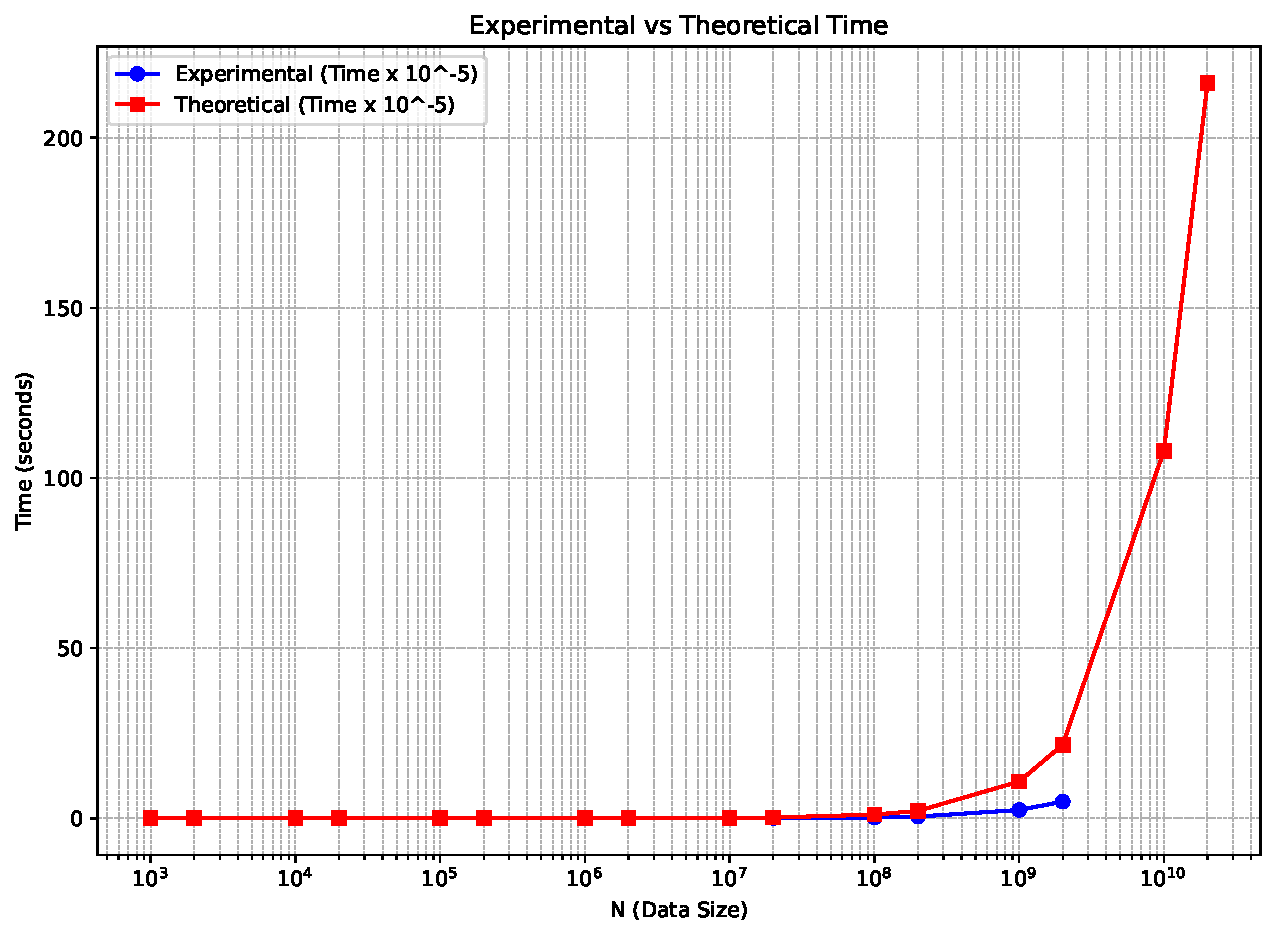
\includegraphics[width=0.85\textwidth]{Questions/Part4/plot.pdf}
    \label{fig:time_plot}
\end{figure}

\newpage

To Draw the plots i used the below python script :

\vspace{1cm}

\lstinputlisting[style=pythonstyle2,inputencoding=utf8]{Questions/Part4/draw.py}

\vspace{1cm}

\begin{prettyBox}{Observation}{greenPlot}
From the plots we notice that the 4th solution takes about the same time as 3rd solution but as n grows bigger the 4th solution takes about
half time of the 3rd therefore the 4th solution is the most efficient out of all the solutions
\end{prettyBox}




\lstinputlisting[style=cstyle]{Questions/Part1/PSUM\_1.c}

\newpage

\section{Transfert Du Fichier Malveillant}

\begin{center}
    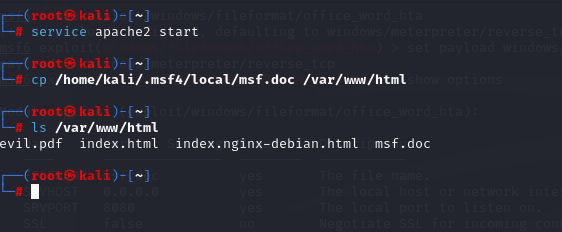
\includegraphics[width=0.8\textwidth]{Question/SC/9_kali.PNG}
\end{center}

\vspace{0.15cm}

\begin{center}
    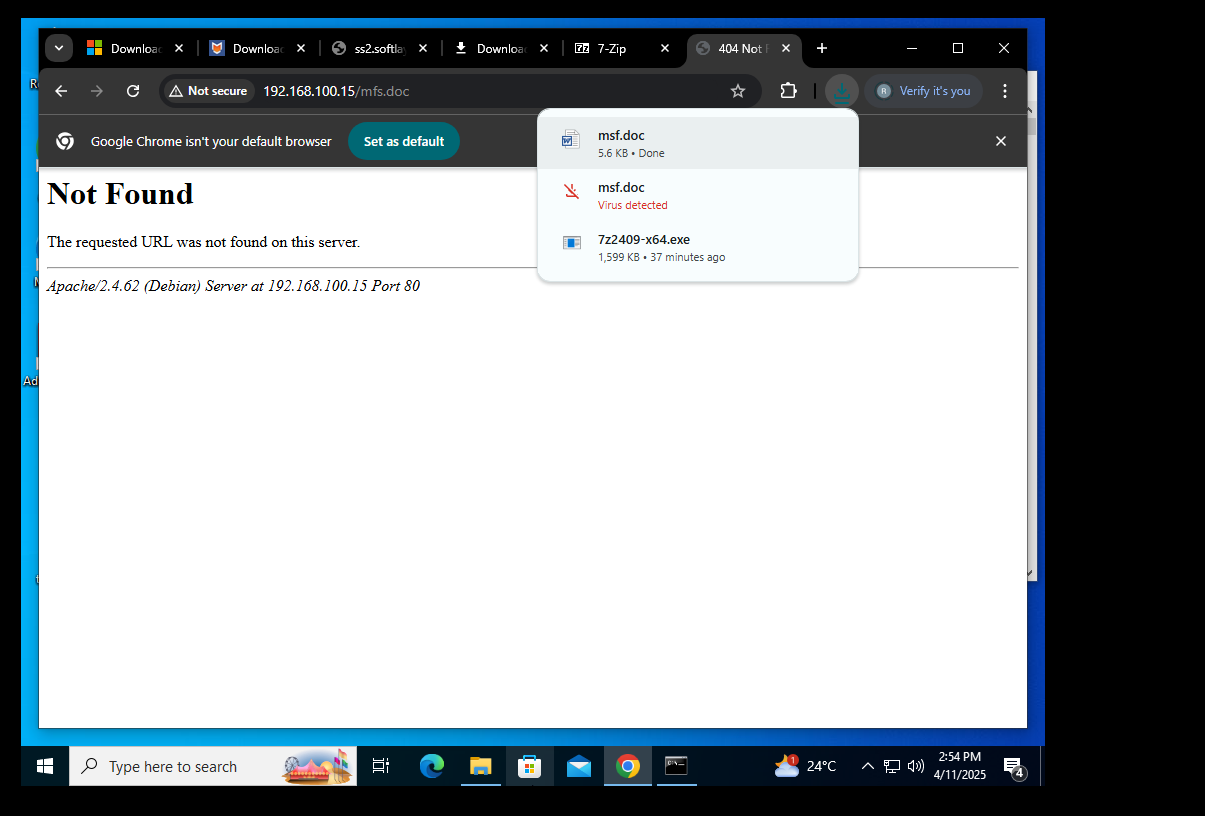
\includegraphics[width=0.6\textwidth]{Question/SC/9_win.PNG}
\end{center}

\vspace{0.15cm}

\begin{center}
    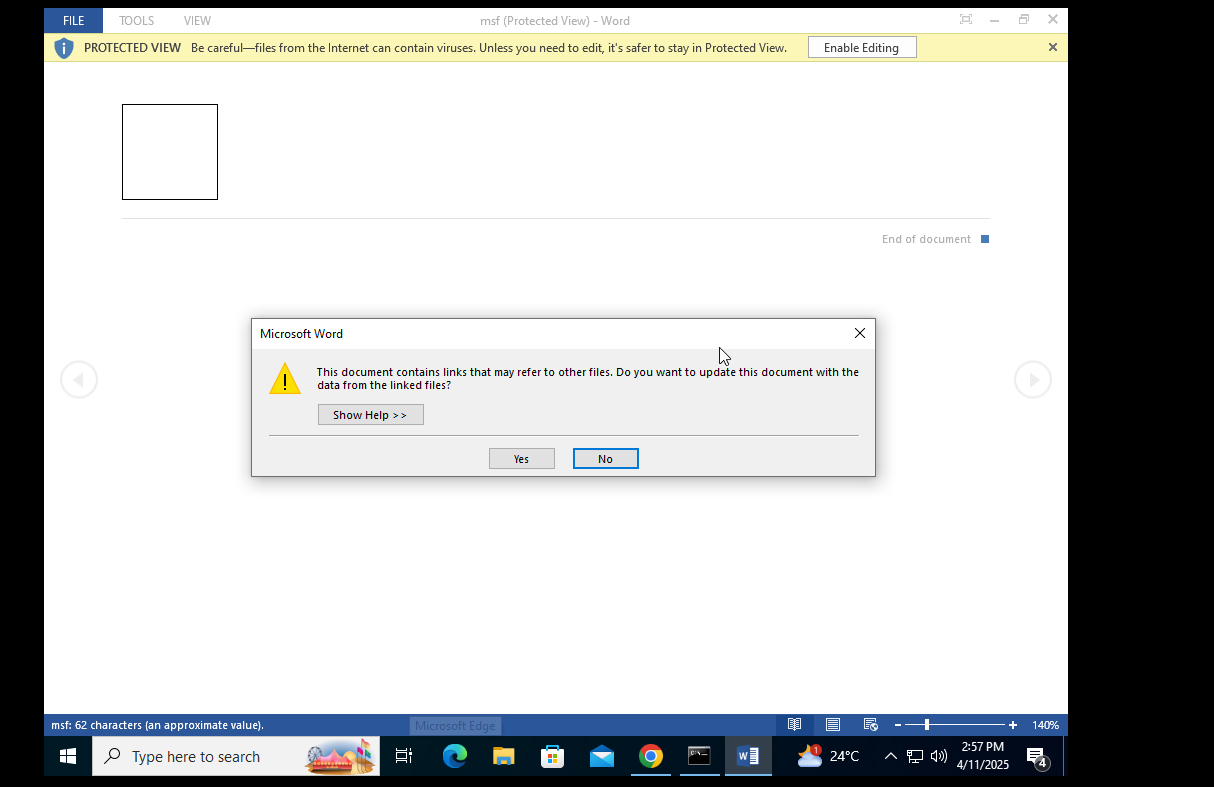
\includegraphics[width=0.6\textwidth]{Question/SC/9_3.PNG}
\end{center}


\vspace{0.35cm}

\begin{prettyBox}{Transfert de fichiers malveillants}{myblue}
\begin{itemize}
    \item On peut transférer le fichier à l'utilisateur sous un nom différent par email, lien, programme qui force l'installation, etc.
\end{itemize}
\end{prettyBox}

\section{Payload \& Handler}

\begin{center}
    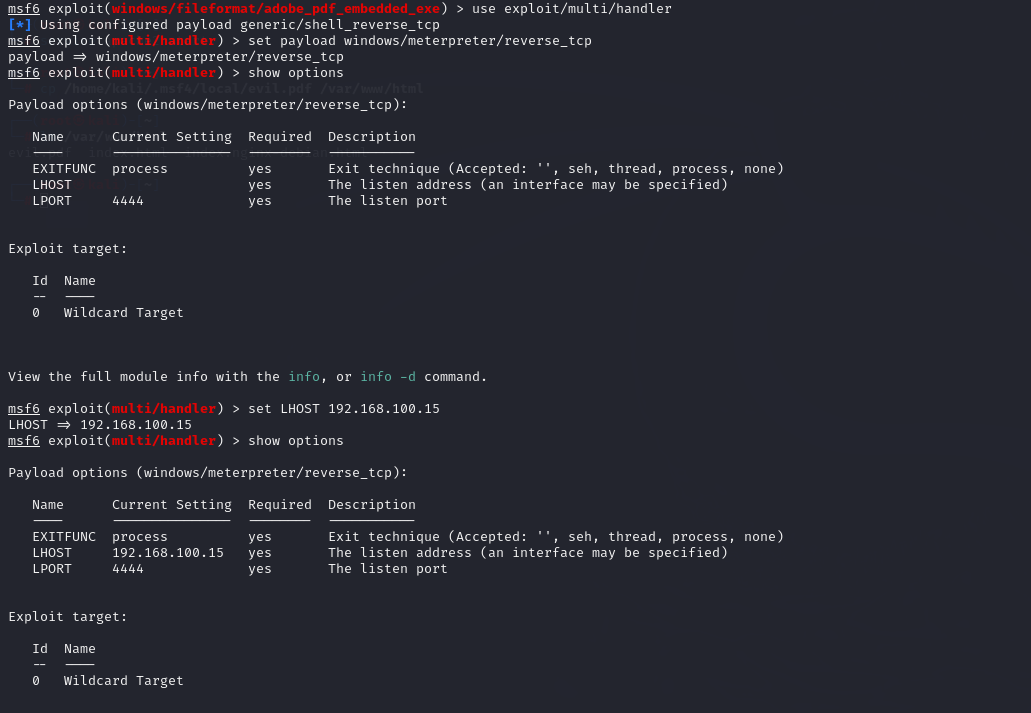
\includegraphics[width=0.8\textwidth]{Question/SC/13_14_15-.PNG}
\end{center}

\vspace{0.15cm}

\begin{center}
    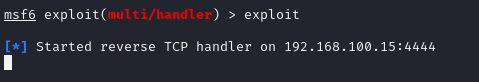
\includegraphics[width=0.6\textwidth]{Question/SC/16.PNG}
\end{center}

\vspace{0.15cm}

\begin{center}
    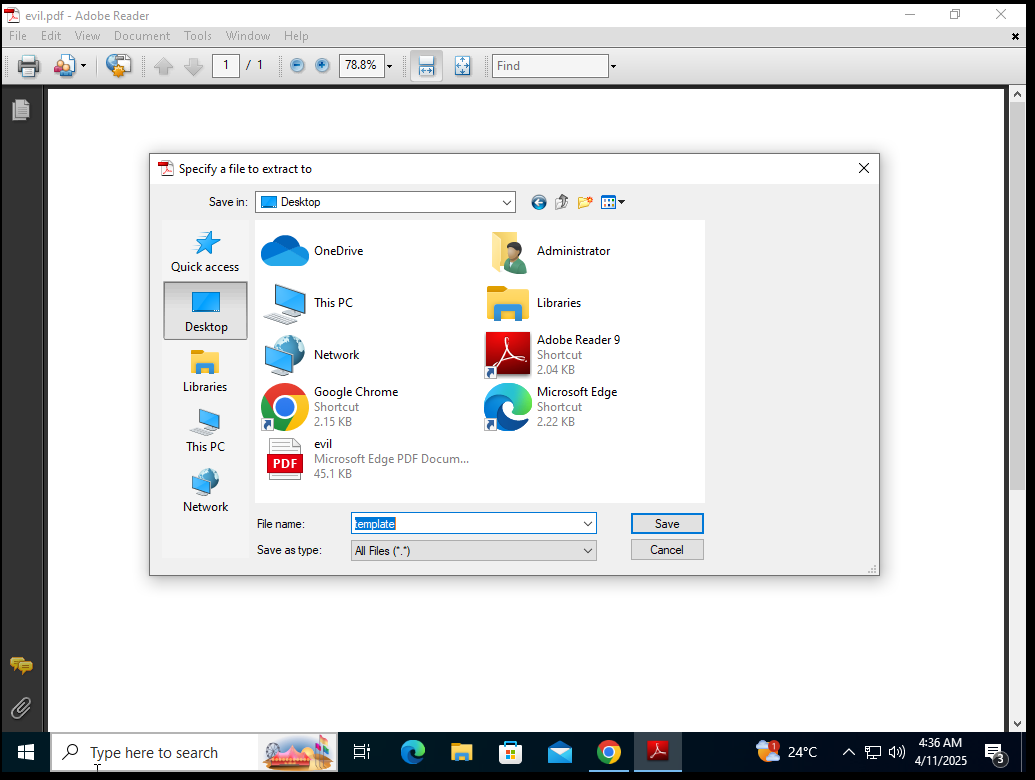
\includegraphics[width=0.6\textwidth]{Question/SC/17.PNG}
\end{center}

\vspace{0.15cm}
\begin{center}
    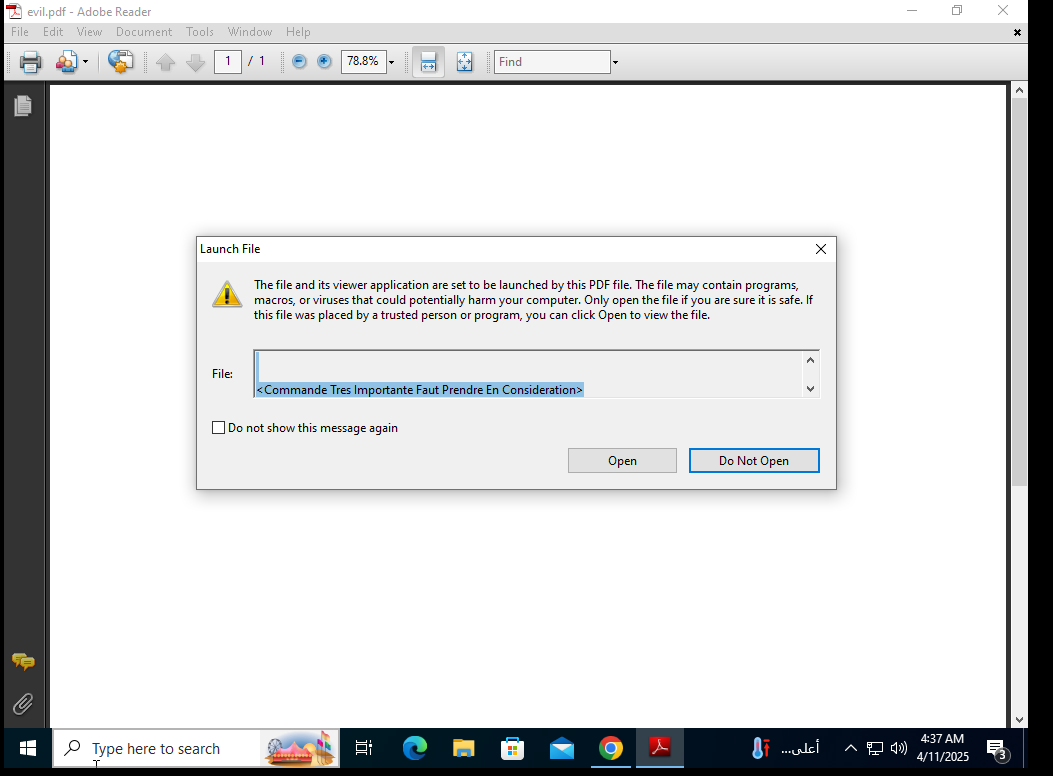
\includegraphics[width=0.6\textwidth]{Question/SC/18.PNG}
\end{center}


\vspace{0.35cm}


\begin{prettyBox}{Définitions Des Termes}{myblue}
    \begin{itemize}
        \item \textbf{Handler} : programme exécuté sur la machine de l'attaquant, qui se met en écoute afin d'attendre une connexion provenant de la victime lorsqu'elle exécute le payload (par exemple, en ouvrant un lien ou un fichier malveillant).
        \item \textbf{Payload} : programme malveillant exécuté sur la machine de la victime suite à une action spécifique réalisée par celle-ci.
        \item \textbf{Reverse Shell} : mécanisme permettant à l'attaquant d'exécuter des commandes shell sur la machine de la victime depuis sa propre machine, en utilisant une connexion TCP inverse initiée par la victime.
        \item \textbf{Message affiché} : message qui apparaît sur la machine de la victime, identique à celui configuré précédemment via la commande \texttt{set LAUNCH\_MESSAGE}.
    \end{itemize}
\end{prettyBox}


\newpage
\section{Reverse\_Shell}

\begin{center}
    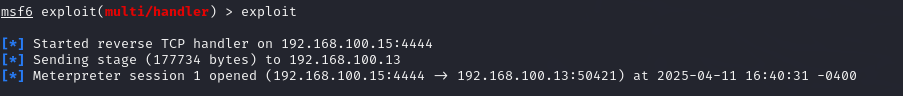
\includegraphics[width=0.8\textwidth]{Question/SC/18_kali.PNG}
\end{center}

\vspace{0.15cm}

\begin{center}
    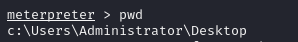
\includegraphics[width=0.6\textwidth]{Question/SC/19_0.PNG}
\end{center}

\vspace{0.15cm}

\begin{center}
    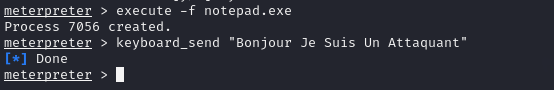
\includegraphics[width=0.6\textwidth]{Question/SC/19.PNG}
\end{center}

\vspace{0.15cm}
\begin{center}
    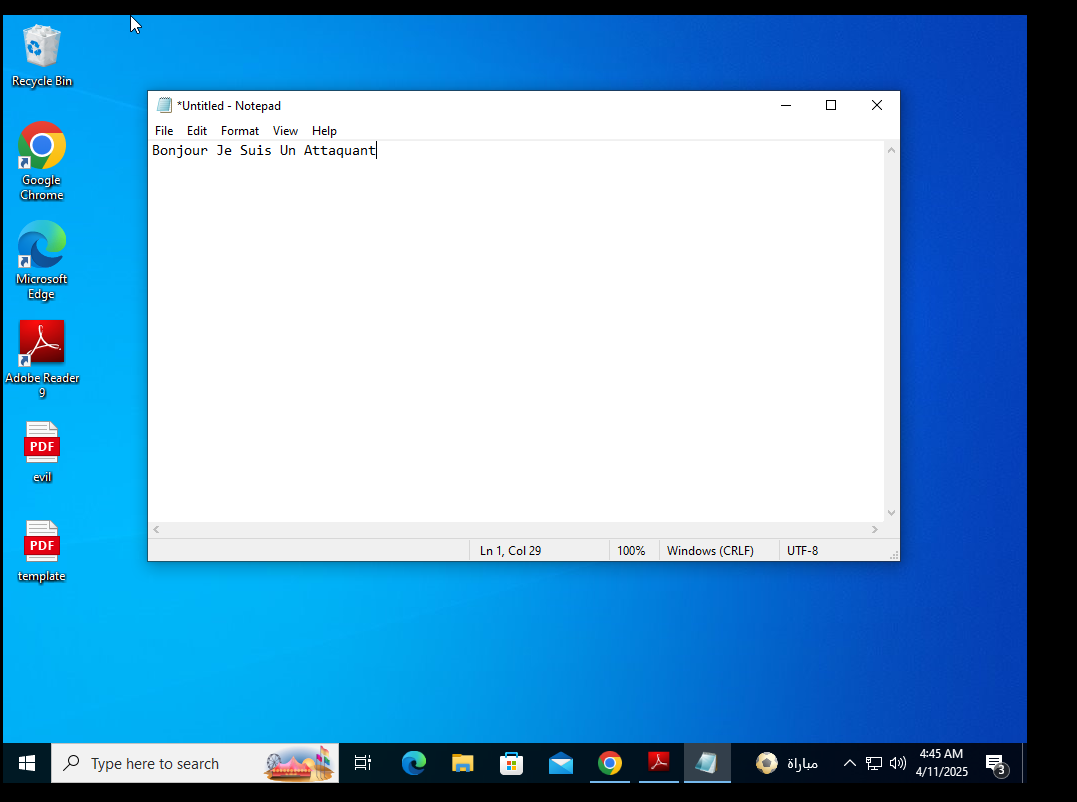
\includegraphics[width=0.6\textwidth]{Question/SC/19_2.PNG}
\end{center}

\vspace{0.15cm}
\begin{center}
    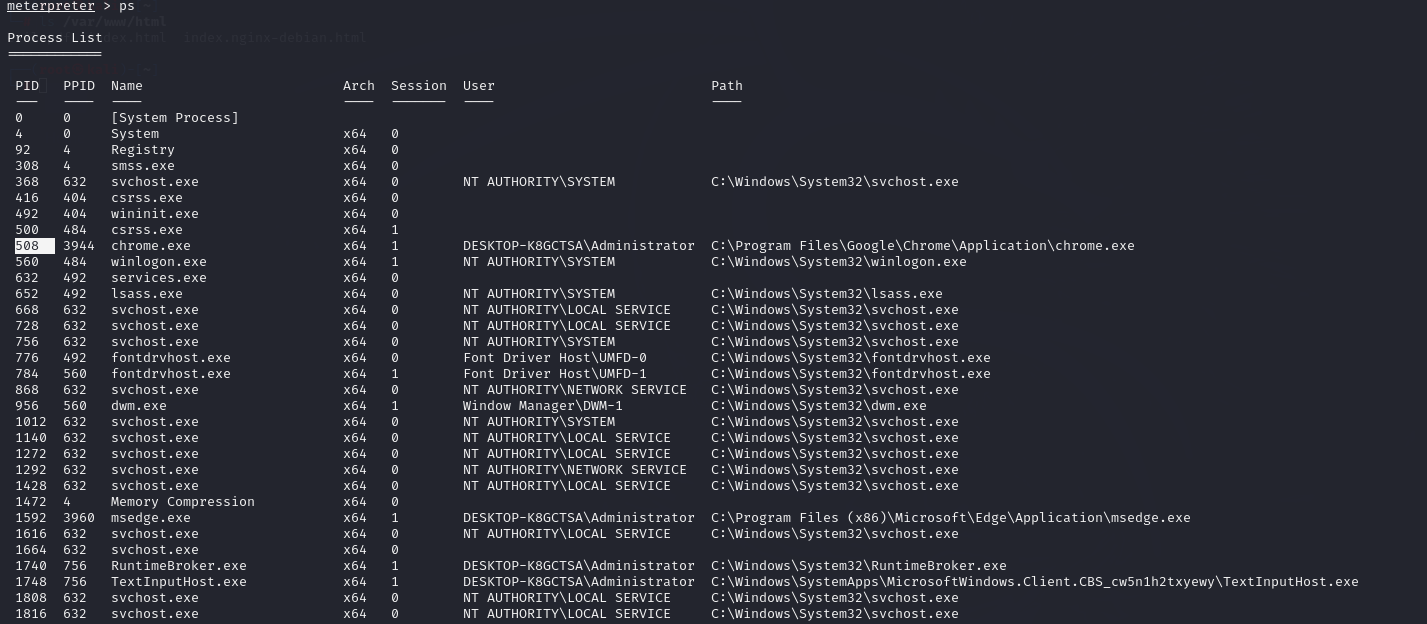
\includegraphics[width=0.6\textwidth]{Question/SC/20_1.PNG}
\end{center}

\vspace{0.15cm}
\begin{center}
    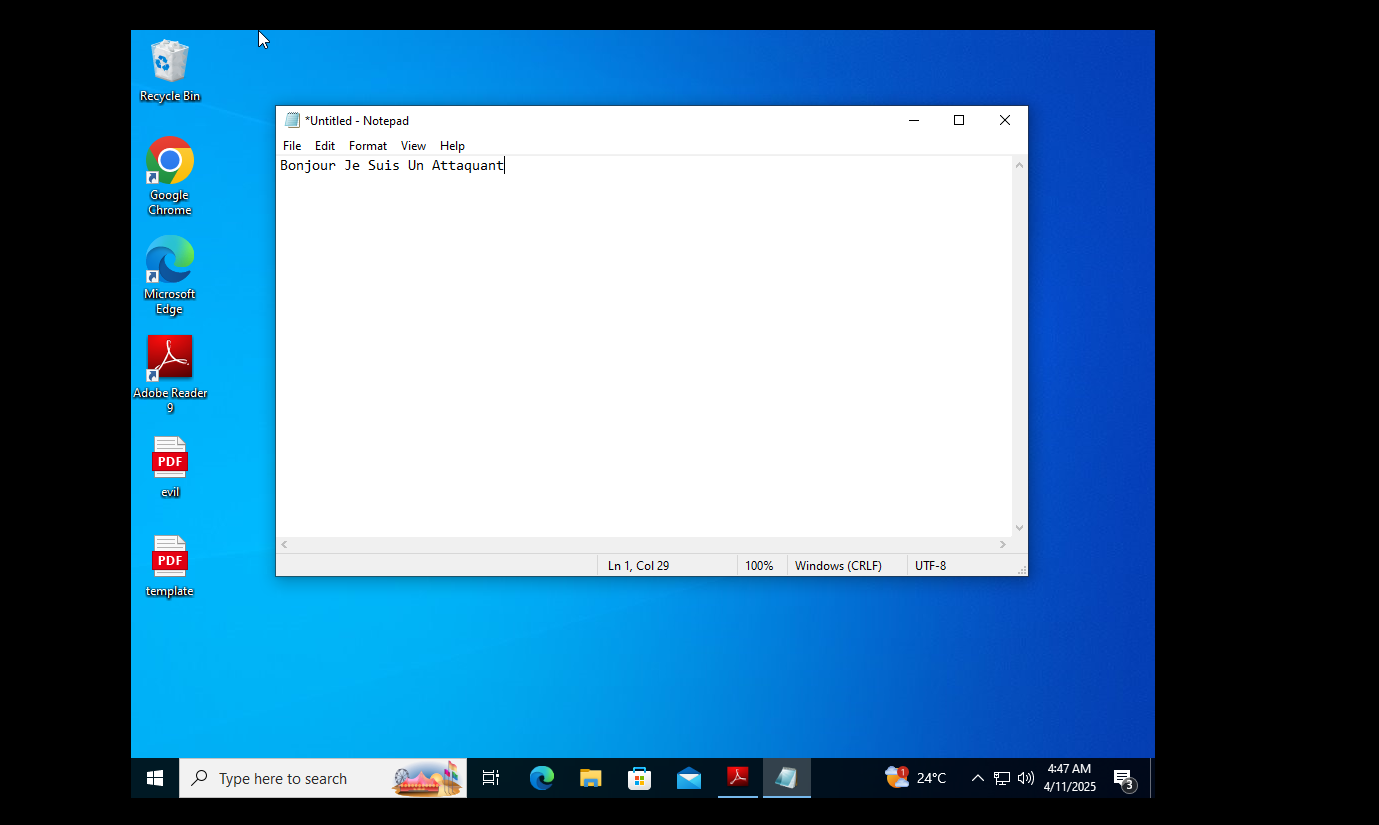
\includegraphics[width=0.6\textwidth]{Question/SC/20_2.PNG}
\end{center}



\vspace{0.35cm}


\begin{prettyBox}{Commandes \& Remarques}{myblue}
    \begin{itemize}
        \item \textbf{Remarque} : Après que l'utilisateur ouvre le fichier \texttt{template.pdf}, le payload s'exécute et l'on peut alors démarrer une session de type \texttt{reverse\_shell}.
        \item \textbf{pwd} : affiche le répertoire courant sur la machine cible.
        \item \textbf{keyboard\_send} : cette commande écrit le message spécifié par l'attaquant directement sur la machine victime. Dans notre cas, le message apparaît dans le bloc-notes (\texttt{notepad.exe}).
        \item \textbf{ps} : affiche les noms, les identifiants (PID), et les chemins d'accès des processus actifs sur la machine cible.
    \end{itemize}
\end{prettyBox}


\end{document}
